\chapter{Propaganda and Populism}
\label{app:prop_and_populism}

In this appendix, we analyse the relationship between propaganda and populism.
This analysis, while slightly drifting away from the core objectives of this thesis, is still related and helps our analysis in Chapter~\ref{ssec:ps_prop_leaning_classifier_conclusion}.

% We have three main objectives:
% \begin{enumerate}
%     \item analyse the conceptual similarities and differences between 
%     \item showing that populisim exists across different political contexts, belonging to different orientations (Left vs Right)
%     \item analyse the correlation between propaganda and populism
% \end{enumerate}
% Relying on the wider literature about populism, we want to see how these two phenomena are related by performing a correlation analysis.
% Being automated propaganda detection a quite recent task, we want to perform this correlation analysis to test our hypothesis that they are related. 
%In this way, we can see if there are some discrepancies between populism existing from all political leanings, an
% if we find that the propaganda datasets are imbalanced while the populism literature shows that 
% If they show to be related, then both propaganda and populism should be distributed in a similar way across the political spectrum.

%\item
% [H2:] propaganda is co-occurring to populism. We need to formulate and verify this hypothesis to then prove or confute H1.

We have three main objectives:

\begin{enumerate}
    \item Analyse the conceptual similarities and differences  between \textit{propaganda} and \textit{populism}: with the findings of the previous point (high imbalance), and given that not much literature exists considering propaganda and political leaning, we need to rely on the concept of populism. %At the same time, we see a lot of publications that refer to a similar concept, populism, that is being observed and studied across countries and political ideologies. 
    We show in this subsection the differences and similarities between these two concepts, and why we hypothesise that they are related (Section~\ref{ssec:ps_prop_leaning_imbalanced_concepts_populism_propaganda}).
    %This supports H2.
    \item Show that populisim exists across different political contexts, belonging to different orientations (Left vs Right).
    We present some contexts where populism is being studied, belonging to different political ideologies and leanings (Section~\ref{ssec:ps_prop_leaning_imbalanced_populism_across}). 
    %This indirectly supports H1, since propaganda is related to populism thanks to the verification of H2, and we show here that populism exists all across the political spectrum.
    \item Analyse the Correlation between detected propaganda and populism: with a dataset that contains speeches with leaning and populism information, we analyse the speeches with propaganda analysis to see the correlation between the detected propaganda techniques against the populism annotations. We do a breakdown by leaning and technique to see where the correlation is stronger (Section~\ref{ssec:ps_prop_leaning_imbalanced_correlation_populism}). 
    %This is a different test of H2, and we present it after the previous point because we are considering \textit{detected propaganda} that is based on an imbalanced dataset.
\end{enumerate}





% In this Appendix we cover the relationship between propaganda and populism.
% This analysis emerged from the analysis of imbalance of Chapter~\ref{chap:political_sides}
% The objectives of this appendix are many:
% \begin{enumerate}
%     \item explain the relationship between populism and propaganda on the conceptual level (Section~\ref{ssec:ps_prop_leaning_imbalanced_concepts_populism_propaganda});
%     \item demonstrate how populism and propaganda are spread around different political context from Left and Right leanings (Section~\ref{ssec:ps_prop_leaning_imbalanced_populism_across});
%     \item study the correlation between populism and detected propaganda (Section~\ref{ssec:ps_prop_leaning_imbalanced_correlation_populism});
%     \item discuss the results and implications of having two related concept, where one of the two (populism) is proved to exist across political leaning and the datasets of the other instead (propaganda) are highly imbalanced (Section~\ref{ssec:ps_prop_leaning_imbalanced_discussion}).
% \end{enumerate}

After facing each of these motivations, we discuss the results and implications of having two related concept, where one of the two (populism) is proved to exist across political leaning and the datasets of the other instead (propaganda) are highly imbalanced (Section~\ref{ssec:ps_prop_leaning_imbalanced_discussion}).

\section{\statusgreen Conceptual Relationship}
\label{ssec:ps_prop_leaning_imbalanced_concepts_populism_propaganda}

To prove the existence of propaganda all across the political spectrum, the best strategy would be to find literature that links propaganda to different political contexts. But, with a bit of surprise, we do not find a lot of literature using the specific term ``propaganda". We have some examples of contexts listed in~\citet{woolley2018computational}, but
most of the socio-political literature uses the concept of \emph{\gls{populism}} that has a much wider systematic theoretical treatment~\citep{muller2017populism,jowett2012propaganda,jowett2018propaganda}. % persuasion (but it has a much larger scope and )
The next Subsection~\ref{ssec:ps_prop_leaning_imbalanced_populism_across} describes therefore the different contexts of propaganda and populism.
%, trying to justify our H1 that propaganda exists in all political leanings.
% Populism is described in different contexts all around the political spectrum, and this is what we will discuss in the next .
But to use the literature of populism for this goal, we need to show how propaganda is related to populism. And this is performed with a theoretical and a practical approach.
We give some theoretical similarities and differences between the concepts in this subsection, and then we will perform a practical correlation analysis in Subsection~\ref{ssec:ps_prop_leaning_imbalanced_correlation_populism}.

% Populism has a very broad systematic theoretical treatment in the literature~\citep{muller2017populism,}

% Populism and propaganda show some similarities and differences, that here in this chapter
% But at the same time, we have a concept that is very closely related with propaganda, that has a very broad systematic theoretical treatment in the literature, that is Populism.

% \todo{duplicate content here and in chapter 2? What is the best place for this?}
As introduced in Chapter~\ref{sec:lit_propaganda} the relationship between populism and propaganda is quite strong~\citep{tumber2021routledge,pasquino2008populism}.


% Definition of Populism
One of the definitions of populism is ``a type of politics that claims to represent the opinions and wishes of ordinary people".\footnote{\url{https://www.oxfordlearnersdictionaries.com/definition/english/populism}}. Many other definitions rely on the concept that populism appeals to ``ordinary people", but it is also true that all politicians appeal to ``the people", wanting to tell a captivating story and be understood.
But populistic is not any successful politician that one does not like.
In~\citet{muller2017populism} there is a stricter definition of populism, and it is based on %gives a quite strong definition of populism all politicians appeal to ``the people" and populistic is not simply any successful politician that one does not like. There are 
two distinctive conditions: it is critical of elites and antipluralist.

On the practical aspect, Populism is often defined on political speeches from political leaders. Most of the existing datasets are a collection of public speeches that come from public representatives.
As an example, we see that~\citet{hawkins2019global} implements populism as a numerical value that is assigned to political speech given by presidents and prime ministers.


% relationship
On the conceptual level, propaganda and populism are two separate concepts. The first describes more the persuasion means used to push for an agenda, while the second one is usually used more together with the actor that wants to push the agenda. 
% And to be on the side of ordinary people, it uses propaganda as a mean to persuade. So a populistic \emph{actor} uses propaganda \emph{techniques}. % Conceptually, they are related.
%
%
%
%
%
% And this computational literature, as discussed in Chapter~\ref{sec:lit_related_populism}, is related to a socio-political literature that is mostly related to the concept of persuasion/manipulation. But at the same time, we have a concept that is very closely related with propaganda, that has a very broad systematic theoretical treatment in the literature, that is Populism.
But the two concepts are linked together by many publications~\citet{tumber2021routledge,pasquino2008populism}: their relationship is very tight even if they have a different role. Populistic \emph{actors} use propaganda \emph{techniques} as a mean to persuade or manipulate the audience.
And given the contemporary digital age, the two concepts are coming closer and closer together, even in democracies, as described in the concept of \textit{rewired propaganda}~\citep{oates2021rewired}. %, we have that in the contemporary digital age, the concepts of propaganda is coming closer and closer to the one of populism, both in non-free states and in democracies.
% At the same time, we see that the literature, especially in socio-political works, refers to a very similar concept, \emph{populism}




\section{\statusgreen Propaganda and Populism across all Political Contexts}
\label{ssec:ps_prop_leaning_imbalanced_populism_across}

In this subsection we show how propaganda (and populism) are spread in contexts across all political leanings. We list the contexts considering the countries and the involved political leanings.
% This backs up H1.

% This subsection’s question: does populism exist in political contexts all across the spectrum?


We start with a few contexts that refer directly to the concept of propaganda~\citep{woolley2018computational}. It is important to notice that in this work, they focus on computational propaganda to mean propaganda that is helped by computational methods in the generation or spread (bots):

\begin{itemize}
    \item Russia: political Parties and State are the major creators of propaganda. RT and Sputnik are the major news sources which have Right-leaning (according to MBFC\footnote{\url{https://mediabiasfactcheck.com/rt-news/}}\footnote{\url{https://mediabiasfactcheck.com/sputnik-news/}}) and are notorious to share the propaganda of the Russian state (extreme-right leaning\footnote{\url{https://mediabiasfactcheck.com/russia-media-profile/}})
    \item Ukraine: the two major sources of propaganda have been, in the recent years, the Russian propaganda on one side, and the counter-propaganda from patriotic Ukraine. A propaganda war, that lives inside the current conflict. And it crosses many times the border between persuasion and misinformation, with many stories shared with the intent to deceive and rewrite the narrative.
    \item Canada: right-wing populism has roots from the 1970s with the \emph{western alienation}~\citep{henry2000revisiting}, and keeps up to recent times with political parties as the \emph{People's Party} which has self-described itself as ``smart populism".
    \item Poland: mainly right-wing is building armies of bot accounts to manipulate social media and online discussions.
    \item Taiwan: this country is in a propaganda war between the mainland Chinese propaganda promoting reunification of the two countries (Left-wing), and the indipendentist propaganda that instead focuses more on internal issues (more Right-wing).
    \item Brazil: also in this country, there are two main forces that drive propaganda. On the Right-wing, the main propaganda figure is Bolsonaro, while on Left-wing the propaganda of Lulism.
    \item Germany: this country historically has seen many types of propaganda, from Nazi propaganda in WWII, anti-communist propaganda during Cold War, evolved to anti-Russian propaganda recently, and also examples of anti-immigration propaganda. Mostly right-wing populist movements.
    \item United States: here, most of the propaganda is linked to the Trump-Clinton election campaigns of 2016, and then propaganda from Trump's presidency. The authors describe mostly the roles of bots in spreading automated campaigns on both sides.
    \item China: the authors study the role of computational propaganda in the state with the ``most sophisticated regime of Internet censorship and control in the world". The findings are that there is little evidence of automation associated with state interests, but anti-state perspectives (pro-democracy movements) are widely automated.
\end{itemize}

Across these examples, we see that most of the propaganda is Right-wing, but we also have examples of Left-wing propaganda (Ukrainian patriotism, Brazilian Lulism, Clinton's liberalism).

But the situation becomes much more balanced with lots of examples when we use the literature related to \gls{populism}.
The term ``populist” has been applied to a heterogeneous group of political groups ranging from the anti-globalization left and greens to the nationalist right.~\citep{kuzio2010populism}.

The work of~\citet{muller2017populism} enumerates different contexts both in the left and in the right. As examples from the Right, Marine Le Pen (France) and Geert Wilders (The Netherlands). As examples from the Left, Bernie Sanders in the US~\citep{postel2016if,jensen2017populism,busby2019framing},\footnote{\url{https://www.oah.org/tah/issues/2016/february/if-trump-and-sanders-are-both-populists-what-does-populist-mean/}} the left-wing alliance \emph{Syriza} in Greece, \emph{Podemos} in Spain (shares with Syriza the opposition to Merkel's authority policies), and then the ``pink tide" in Latin America: Raphael Correa (Ecuador), Evo Morales Bolivia), Hugo Chávez (Venezuela).

As additional resources, we also point at Wikipedia that contains a list of countries both for Left\footnote{\url{https://en.wikipedia.org/wiki/Left-wing_populism\#By_country}} and Right\footnote{\url{https://en.wikipedia.org/wiki/Right-wing_populism\#Contemporary_movements_by_country}} wing populism.


With the examples provided, we have demonstrated that populism (and propaganda as they are linked) are spread all across the political spectrum.

\section{\statusgreen Correlation between Populism and Detected Propaganda}
\label{ssec:ps_prop_leaning_imbalanced_correlation_populism}

% explain Why?
Having noticed the imbalance of the propaganda datasets in~\ref{ssec:ps_prop_leaning_imbalanced_datasets} and the ubiquitousness of populism in~\ref{ssec:ps_prop_leaning_imbalanced_populism_across}, we want in this subsection to analyse the correlation between populism and the detected propaganda.
% need to verify or refute our hypothesis about the correlation between populism and propaganda.

Even if propaganda here is \textit{detected} using imbalanced datasets, we hypothesise that, to some limitations, these datasets are able to detect some propaganda over the Left and Center. This last hypothesis is somewhat confirmed by the above Section~\ref{ssec:ps_prop_leaning_across} that found that we have some outputs that make sense from applying propaganda detection on different political leanings.
These results may not be highly accurate, but they can help us solve this circular dependency (accurately detect propaganda $\rightarrow$ demonstrate correlation between propaganda and populism $\rightarrow$ demonstrate propaganda datasets should include more left-leaning $\rightarrow$ accurately detect propaganda) and give a first approximative result.

We need to understand the magnitude of this correlation because we are facing a discrepancy between populism (all across leaning) and propaganda datasets (mainly right-leaning).
We hypothesised the correlation between propaganda and populism, but we need to actually analyse it.

We also have a secondary objective for this section: studying where the correlation is stronger and where it is weaker could help us analyse potential areas where propaganda detection is not working well. In other words, if we observe that for a specific leaning and technique, the correlation is low/negative, this could be an indication that the propaganda detection for that leaning and technique is not accurate.

% On the experimental side, we need to verify our assumption, that we took from the literature, of \textit{the correlation between propaganda and populism}

% Populism vs propaganda: seen before in

% The term ``populist” has been applied to a heterogeneous group of political groups ranging from the anti-globalization left and greens to the nationalist right.~\citep{kuzio2010populism}

% setup
Therefore, we proceed with this experiment with the following setup:

\begin{itemize}
    \item identify a dataset which contains both information about populism and political leaning;
    \item annotate such dataset with propaganda techniques;
    \item perform correlation analysis between populism scores and detected propaganda techniques.
\end{itemize}

% dataset
After looking at the available datasets for populism, we selected the dataset from~\citet{hawkins2019global} because it is quite balanced in terms of the political orientation of the actors annotated. % (liberal vs conservative, since it is US-based).%\todoAW{It strikes me here that this is a very US-centric interpretation of the political landscape. Do you consider whether the make up of the dataset poses any threats to validity?}
It contains 1240 political speeches, from several countries and languages.
For each one of them, there are four annotators that give a numerical score of populism in the range $[0;2]$ where $0$ means non-populistic and $2$ means very populistic. The single annotations are already averaged out.
So from the 4961 raw rows, by deduplicating (4 annotations for each speech) we have 1240 speeches, out of which 265 are in English (then down in the rankings, 304 in Spanish and 148 in Portuguese).
These 265 speeches all have a leaning classification (we will see more about leanings in the next chapter): 36 Left, 37 Center, 84 Right, 106 NA. We use this information in order to check whether the results that we get are general across the political spectrum.

% annotation of the dataset
We run this dataset through the propaganda annotation tool~\citep{da2019fine}, to detect the specific propaganda techniques that have been used.
We rely on two metrics that we already used in the previous sections: the total quantity of propaganda in each article and the quantity of each propaganda technique, as word-based percentages. We exclude the term analysis because the populism annotations are only at the speech level and not at the word-level. % Not words? Term analysis?

% correlation as Spearman's correlation
For the correlation, we want to compute how much propaganda and populism are strictly related. So we take each speech in the corpus and we proceed to compute the Spearman's correlation~\citep{spearman1910correlation} between the  populism averaged out between the annotators and different propaganda metrics: total word-based percentage of propaganda, and word-based percentage of each of the propaganda techniques. 

% first overall
% then breakdown by political leaning
We first analyse these correlation metrics on the overall dataset, then we break down the analysis considering the labels of the political leaning of the articles.


\subsection{Correlation between Propaganda and Populism}
% TODO bring \ref{ssec:lp_techniques_populism_vs_propaganda} here

% from "Propaganda datasets imbalanced?"
% What
% In this section, we experiment with another concept from the literature that is shown to be close to persuasion and propaganda: \gls{populism}~\citep{tumber2021routledge,pasquino2008populism}. %\todoHA{Not mentioned in intro. Why not?}
% We want to understand: what is the substantial difference between populism and propaganda? Can these two phenomena be related?

% why
% We need to understand the magnitude of this correlation because here in this section we are showing a discrepancy between populism (all across leaning) and propaganda datasets (mainly right-leaning).
% We hypothesise the correlation between propaganda and populism, but we need to actually analyse it.
% This question arises purely from a logistical point of view: we have automated methods for detecting propaganda, but we do not have tools to detect populism.
% Therefore, if we can prove that populism and propaganda are actually correlated, then it becomes not important for us to be able to detect something that is very much correlated to something else that we already detect.

% \todoHAinline{ok, but what would detecting populism give you? Why is this of value?}

% \todoHAinline{I would start by: 1. explaining value of detecting populism. 2. detecting it and evaluating that, then 3. see if correlated with propaganda}

% practically/computationally
% On the computational/detection side, we want to see if this relationship between populism and propaganda stands.
% So to evaluate it, we have computational approaches for propaganda detection, but not for populism detection.
% A solution to this problem, is to use a dataset where we have the ground truth for the populism, which will be run through the propaganda detection pipeline. Then we will compute the correlation between the two, and we can establish whether this relationship is proven. The advantage of using directly the ground truth for one of the two phenomena (populism) is that we can only have errors for the propaganda detection.\todoHA{unclear} Instead, if we were to compare two predictions, the errors could be on both sides.

% % dataset used
% For this experiment, after looking at the available datasets for populism, we selected the one from~\citet{hawkins2019global} because it is quite balanced in terms of the political orientation of the actors annotated (liberal vs conservative).\todoAW{It strikes me here that this is a very US-centric interpretation of the political landscape. Do you consider whether the make up of the dataset poses any threats to validity?}
% It contains 1240 political speeches, from several countries and languages
% For each one of them there are four annotators that give a numerical score of populism in the range $[0;2]$ where $0$ means non-populistic and $2$ means very populistic. The single annotations are already averaged out.
% So from the 4961 raw rows, by deduplicating (4 annotations for each speech) we have 1240 speeches, out of which 265 are in English (then down in the rankings, 304 in Spanish and 148 in Portuguese).

% These 265 speeches all have a leaning classification (we will see more about leanings in the next chapter): 36 left, 37 center, 84 right, 106 NA. We use this information in order to check whether the results that we get are general across the political spectrum.


% Dataset found: populism in political speeches %https://dataverse.harvard.edu/dataset.xhtml?persistentId=doi:10.7910/DVN/LFTQEZ&version=2.0 
% Each annotator (4 for each speech) gave a score between 0 (non-populistic) to 2 (very populistic)
% 4961 rows 
% 1240 deduped (352 left, 256 center, 469 right, 652 NA)
% Languages: 265 en (304 es, 148 pt, …),
% Leaning of the english ones: (36 left, 37 center, 84 right, 106 NA)



% Goals:
% With this dataset, as we described, we want to compute the 
% correlation between propaganda and populism. So we take each speech in the corpus and we proceed to compute the Spearman's correlation~\citep{spearman1910correlation} between the  populism averaged out between the annotators and different propaganda metrics: total word-based percentage of propaganda, and word-based percentage of each of the propaganda techniques. 


% results
The Spearman's correlation between the populism and the total word-based percentage (all techniques together) is $0.1694$. This value is quite low. So it seems that they are quite unrelated. %\todoAW{This feels to me like the sort of investigation and analysis which forms the bedrock of your research. So I think you need to set it out more formally so that it feels like less of an aside.}

\begin{figure}[!htbp]
    \centering
    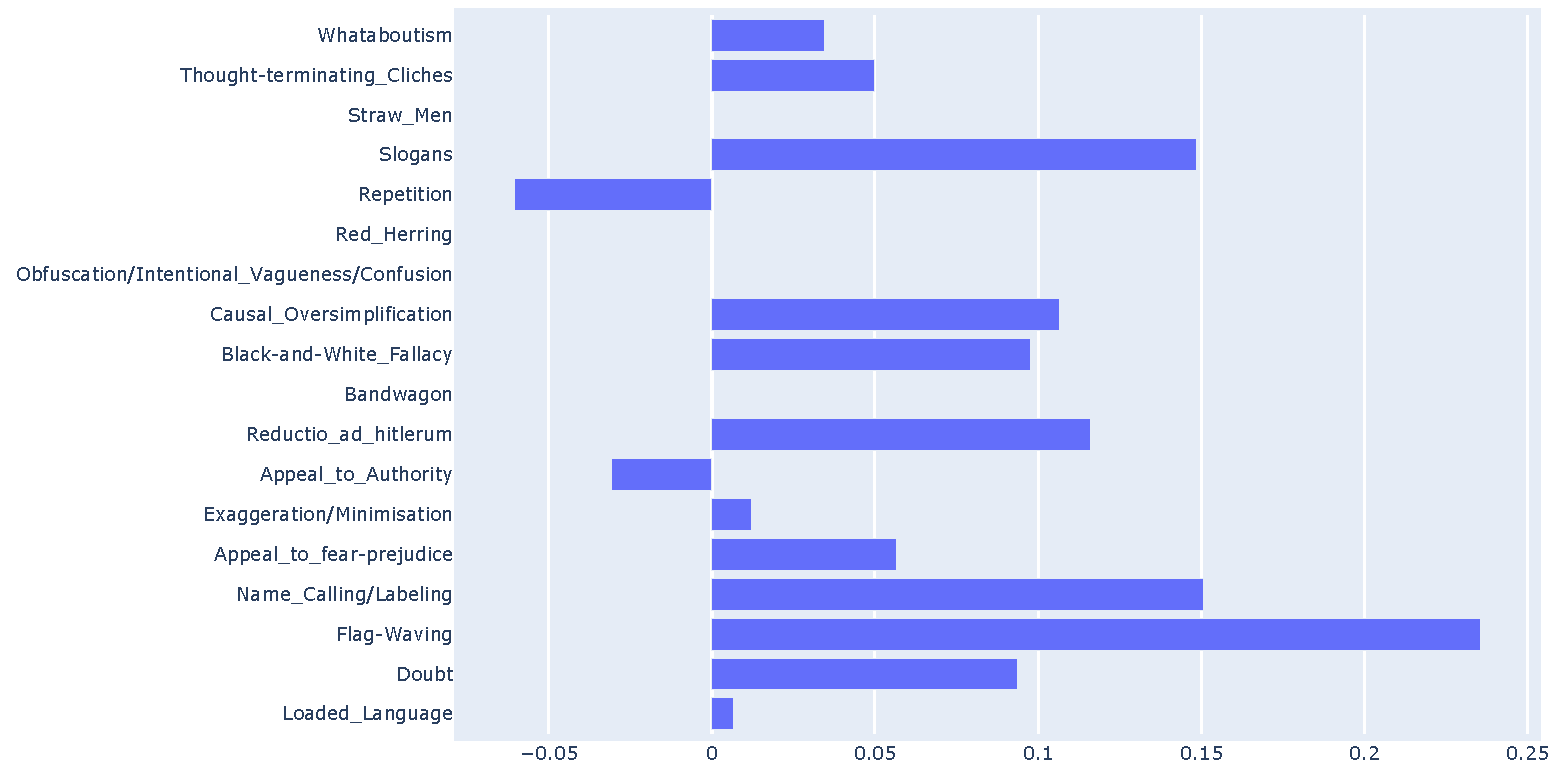
\includegraphics[width=\linewidth]{figures/populism_propaganda_correlation.pdf}
    \caption{Correlation between populism and each propaganda technique.}
    \label{fig:populism_propaganda_correlation}
\end{figure}

By breaking it down to the correlation of populism to each propaganda technique, we can see in Figure~\ref{fig:populism_propaganda_correlation} that the strongest correlation is found with \texttt{Flag-waving}, \texttt{Name\_Calling/Labeling} and \texttt{Slogans}. Some of the techniques have very low correlation. It is interesting to notice that two techniques have slightly negative correlation (\texttt{Repetition} and \texttt{Appeal\_to\_Authority}), so this means that they are used by less populistic speeches.


% L/R evaluation:
% Assumption: propaganda correlates to populism similarly in L/C/R
% Result total: 0.225 Left, 0.005 Center, 0.374 Right → Why? Is it a matter of quantity of populism/propaganda?
% Populism average:  [0.1259, 0.0729, 0.2712]
% Propaganda average: [0.0165, 0.0271, 0.0432]
% Ratio: [0.1317, 0.3717, 0.1593] → populism over propaganda ratio is a bit bigger on the right (21\% more), but the correlation Right is bigger than the left at 66\%. So it is less likely that this is just a matter of quantity. On the Right, propaganda and populism are strongly linked

% findings
Propaganda and populism are correlated, but not too strongly.
The fact that some of the techniques are correlated to populism is a good sign. Even though, the correlation scores are still low to be considered as ``strong correlation''. We will expand this experiment in the next Chapter when we take into consideration political leaning.
Considering that the current fine-grained propaganda detection is not so accurate (cf. Section~\ref{ssec:lp_techniques_propaganda}), we can say that this weak correlation can still be considered as a signal that the two phenomena are related.
% In the Right more. This is one point supporting the hypothesis that propaganda detection works better in the Right than in the Left. → imbalanced detection caused by imbalanced data


\subsection{Correlation by Political Leaning}
% This is the continuation of Section~\ref{ssec:lp_techniques_populism_vs_propaganda} from the previous chapter. 
Now we introduce the leaning and %the problem of imbalance, we are going to 
break down the analysis with respect to the political leaning of the speeches.
% Dataset found: populism in political speeches %https://dataverse.harvard.edu/dataset.xhtml?persistentId=doi:10.7910/DVN/LFTQEZ&version=2.0 
% Each annotator (4 for each speech) gave a score between 0 (non-populistic) to 2 (very populistic)
% 4961 rows 
% 1240 deduped (352 left, 256 center, 469 right, 652 NA)
% Languages: 265 en (304 es, 148 pt, …),
% Leaning of the english ones: (36 left, 37 center, 84 right, 106 NA)

These 265 speeches all have a leaning classification: 36 left, 37 center, 84 right, 106 NA. We use this information in order to calculate separately the correlations.


% RESULTS
When we consider populism and the total amount of propaganda, without differentiating by techniques, we get the results shown in Figure~\ref{fig:populism_propaganda_quantities_by_leaning}. The blue bars represent the average of the scores given by the annotators (range $[0;2]$), the red bar instead are the word-based ratio of propaganda (range $[0;1]$) and the green bars are the Spearman's correlations (range $[-1;1]$).

\begin{figure}[!htbp]
    \centering
    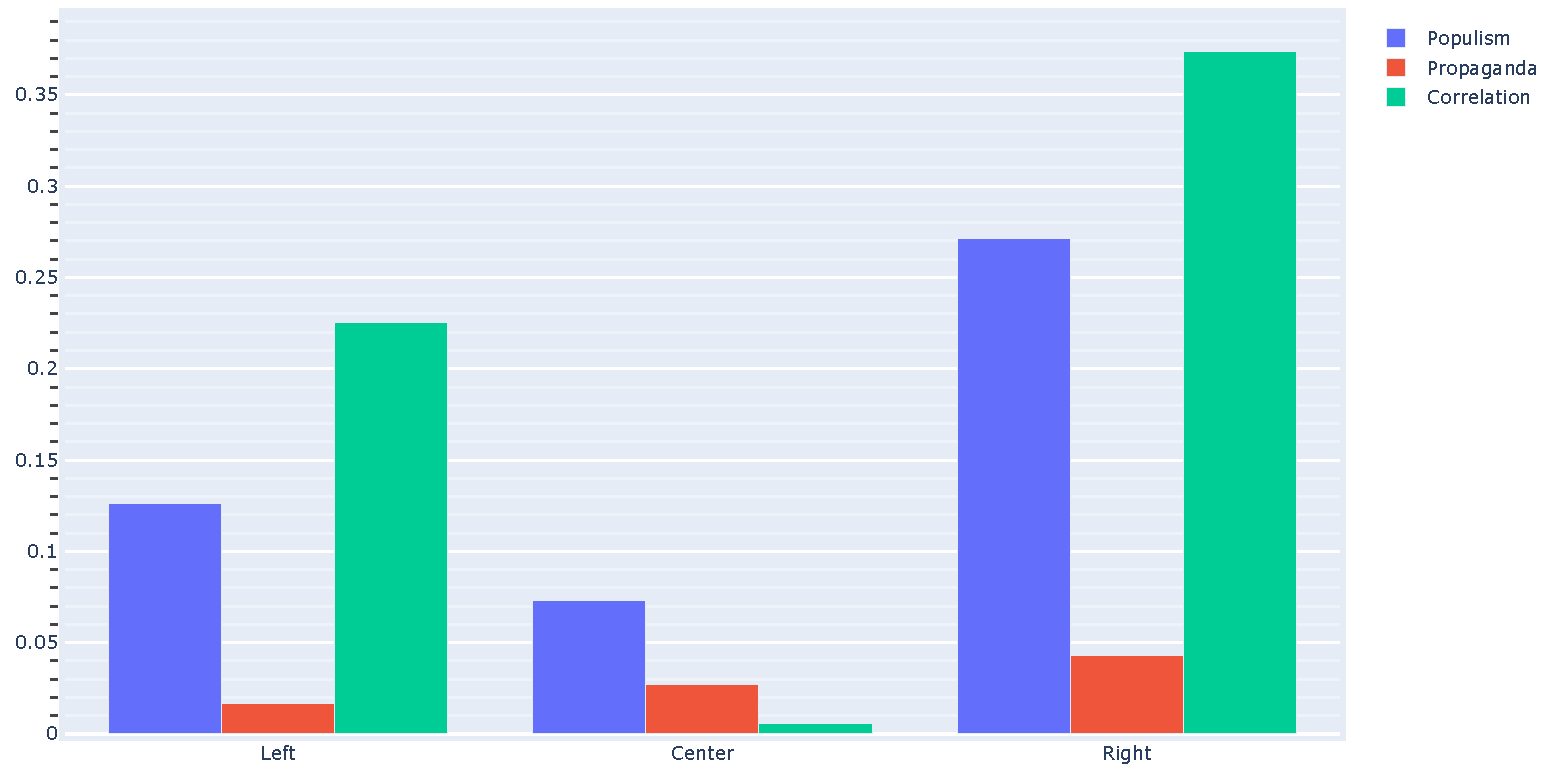
\includegraphics[width=\linewidth]{figures/populism_propaganda_quantities_by_leaning.pdf}
    \caption{Quantity of populism, propaganda and their correlation across leaning.}
    \label{fig:populism_propaganda_quantities_by_leaning}
\end{figure}

We can, first of all, notice that there is more populism and more propaganda in the Right leaning.
While Populism has a \emph{U-shape}, with lower values in the Center, Propaganda has a triangular Right shape, with the values monotonically increasing from Left to Right.

The correlation instead is the one that changes the most: it has its maximum value of 0.374 in the Right, a lower value of 0.225 in the Left, and it is almost zero (0.005) in the Center.
% \begin{itemize}
%     \item 0.225 for speeches in the Left
%     \item 0.005 for speeches in the Center
%     \item 0.374 for speeches in the Right
% \end{itemize}
This means that for the speeches in the Center, populism and propaganda behave in completely independent ways, if we consider all propaganda techniques together.
The value for the Right represents still a weak correlation, but we cannot dismiss it either as ``non-correlated".

% We see that the correlation is higher in the Right leaning.

% Result total: , ,  → Why? Is it a matter of quantity of populism/propaganda?
% Populism average:  [0.1259, 0.0729, 0.2712]
% Propaganda average: [0.0165, 0.0271, 0.0432]
% Ratio: [0.1317, 0.3717, 0.1593] → populism over propaganda ratio is a bit bigger on right (21\% more), but the correlation Right is bigger than left of 66\%. So it is less likely that this is just a matter of quantity. On the Right, propaganda and populism are strongly linked

We then proceed to combine the previous breakdown by propaganda technique with the breakdown by leaning. In this way, we can see how specific propaganda techniques correlate across the political spectrum.

\begin{figure}[!htbp]
    \centering
    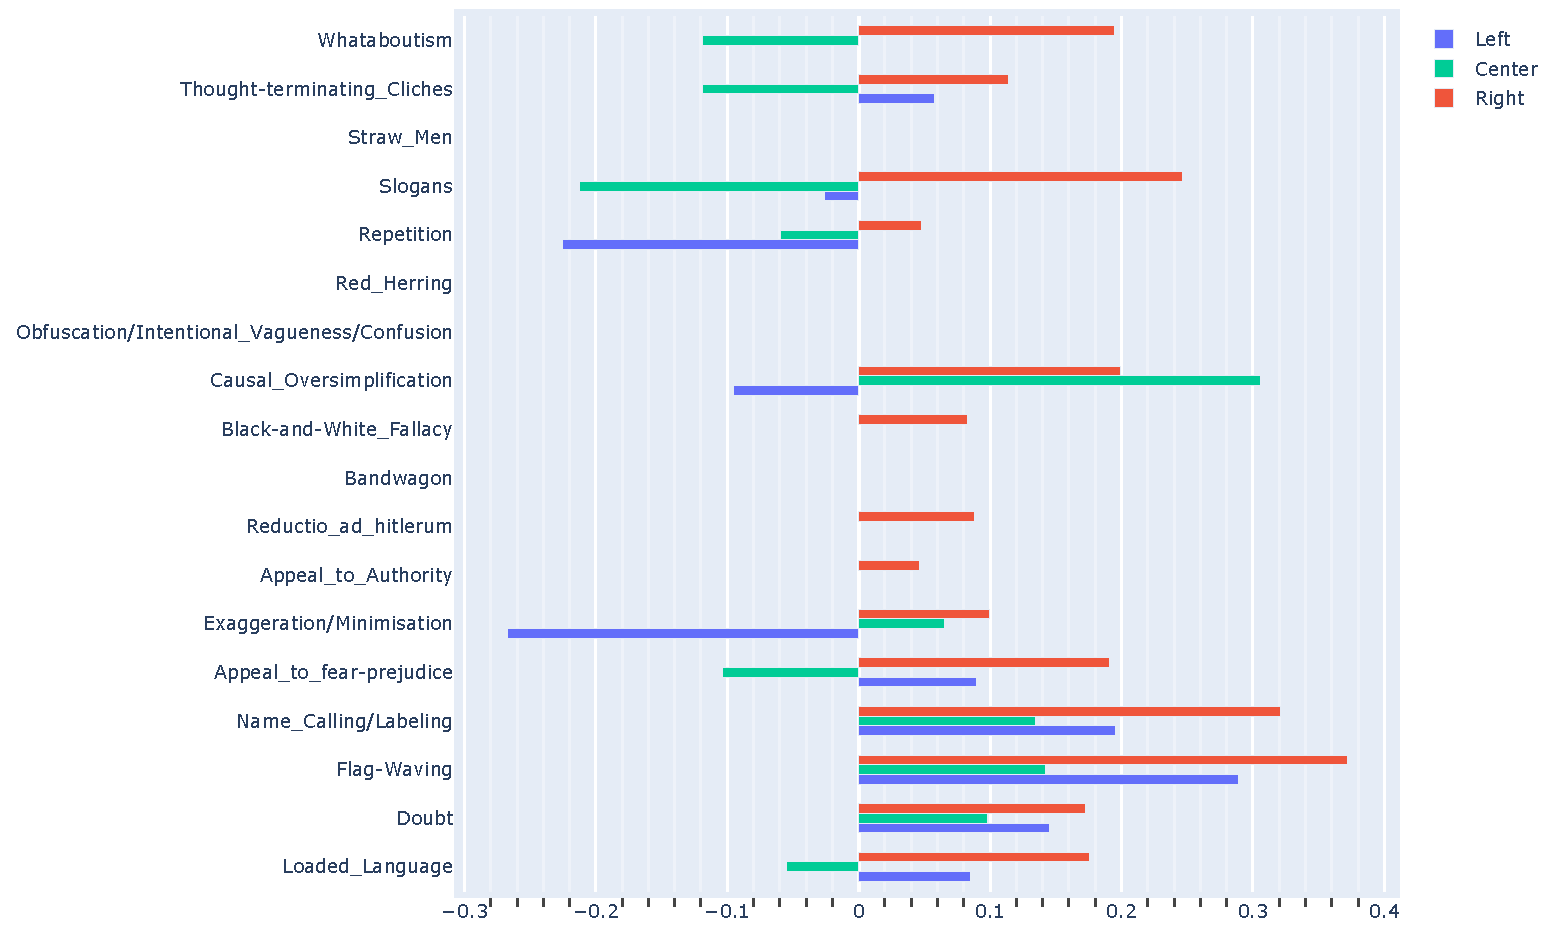
\includegraphics[width=\linewidth]{figures/populism_propaganda_correlation_by_leaning.pdf}
    \caption{Correlation between populism and propaganda techniques across leaning.}
    \label{fig:populism_propaganda_correlation_by_leaning}
\end{figure}

Figure~\ref{fig:populism_propaganda_correlation_by_leaning} shows the breakdown by each technique considering the political leaning of the speeches.

We can see that for some techniques, the values vary a lot across leaning. For example, let us consider the technique \texttt{Exaggeration/Minimisation}. In the right it has a positive value, while in the left it has a negative value. %, and in the center more neutral values.
In other words, populism is correlated positively with this technique in right-leaning speeches, while it is negatively correlated in left-leaning ones. We have this type of behaviour also with \texttt{Repetition}, \texttt{Slogans} and \texttt{Causal\_Oversimplification}. This means that these techniques correspond more to the populism of the right, while are used in the Left in relatively non-populistic speeches.
%(hypothesis H2 of positive correlation broken).
Or it could also mean that the detection of these techniques in the Left is not working as it should.
%(and actually the hypothesis H2 of positive correlation is still valid).

Instead, the techniques \texttt{Name\_Calling/Labeling}, \texttt{Flag-Waving} and \texttt{Doubt} have positive correlations for all political leanings.
Therefore, the detection of these techniques is probably working more accurately as it reflects the expected behaviour (positive correlation).

\section{Results and Discussion}
\label{ssec:ps_prop_leaning_imbalanced_discussion}

Considering the previous subsections, we discuss here the main findings of this investigation.

% \begin{enumerate}
%     \item the conceptual similarities and differences between propaganda and populism
%     \item populism across many contexts of the left and right
%     \item propaganda dataset showing highly imbalanced resources for the English language
%     \item correlation between propaganda and populism that confirms a relationships but for some techniques it shows null or negative correlation to 
% \end{enumerate}


% we have the following points:
% Findings
% We wrap up our main findings of this investigation.

1. Computational NLP resources are quite imbalanced, especially the English based. The main motivation is that most of the works consider as a starting resource MBFC which has a label ``propaganda" that is on the limit of fake news, which is associated with extreme leanings, and it is more common in the extreme-right leaning with fewer sources on the extreme-left leaning. The datasets derived from MBFC, by selecting the news sources, end up in under-representing of left-leaning and centre, with the result of being completely imbalanced.
At the moment, there are not many datasets available for propaganda detection, and therefore this problem is showing more.
The answer to RQ3.3 is that \emph{propaganda detection is highly imbalanced. The imbalance comes from the datasets that currently only contain right-leaning examples}.
And the results seem to disagree with our hypothesis that propaganda exists all across the political spectrum.
But in reality, what we really observe is that the datasets are imbalanced. Therefore, we want to show some literature that places propaganda all across the political spectrum, to then be able to say that this imbalance should not be there.


2. In our digression over literature, we find that most of the works use a term that is not propaganda: it is populism. Therefore, we analyse the conceptual similarities and differences, to argue that we can use the literature about populism to derive the distribution of propaganda.
% Distinction of terminology: socio-political works tend to use more the populism terminology. 
We find that the concepts are very strictly linked and the main difference is the role: political figures are labelled as populist and the linguistical means they use are in many case propaganda techniques. The term populism focuses more on public figures, while propaganda is more related on the linguistic means.
But we only want to use the concept of populism to understand how it (and propaganda) spread across the political leaning, so we are not interested in this difference. We are only interested in their co-occurrence (when one is present, also the other one).
%And literature supports us and we verify our H2.
% Focus is less on the linguistic means, it is more about the ideals expressed. And populism is more from the political leaders of a position (political speeches).
% Instead, on the NLP side, focus has been more on the propaganda terminology, with some references to persuasion. And propaganda is seen more as related to news sources instead of political leaders.

3. %We then proceed to the verification of 
%using Populism as an intermediary. 
We take the socio-political literature and we find examples of populism all across political ideologies and leanings.


4. We then perform the Correlation analysis and find a weak (but existing) correlation.
% The most correlated techniques are: X Y Z.
More correlation is shown in Right-leaning speeches as a consequence of propaganda being trained on right-leaning sources. But we are still able to detect weaker correlation with propaganda on the Left and Center.
We also find that some techniques have negative correlation with populism. For example \texttt{Repetition} and \texttt{Exaggeration/Minimisation} with articles from the Left, or \texttt{Whataboutism} \texttt{Thought-terminating\_Cliches} \texttt{Slogans} and \texttt{Appeal\_to\_fear-prejudice} with articles from the center.
This may be one of the first noticeable consequences of having imbalanced data for training automated propaganda recognition, indicating that the detection in these situations is not working as expected.
This provides a useful insight for future research that wants to improve propaganda detection.


